\documentclass[12pt]{article}
\usepackage[utf8]{inputenc}
\usepackage{tgbonum}
\usepackage[a4paper, total={6in, 10in}]{geometry}
\usepackage{graphicx}
\usepackage{minted}
\title{Lab Assignment 1}
\author{Akshat Mittal - 20107}
\date{May 2021}
\begin{document}
\maketitle
\vspace{7mm}
\textbf{Contents}
\vspace{7mm}
\begin{enumerate}
    \item Volume of Cube
    \item arithmetic calculations
    \item Use of $sizeof()$ function
    \item 
        \begin{enumerate}
            \item Arithmetic Operators
            \item Assignment Operators
            \item Relational Operators
            \item Logical Operators
            \item Bitwise Operators
        \end{enumerate}
    \item Area of triangle
    \item Simple and Compound interest
    \item Address of the user
    \item Salary, basic pay, HRA and TA
    \item floating numbers in exponential form with decimal precision
    \item Swapping values of two variables
\end{enumerate}
\newpage
\section{}
\subsection{Algorithm}
\begin{enumerate}
    \item Calculate volume by h * w * d
    \item Print volume
\end{enumerate}
\subsection{Flowchart}
\begin{figure}[h]
    \centering
    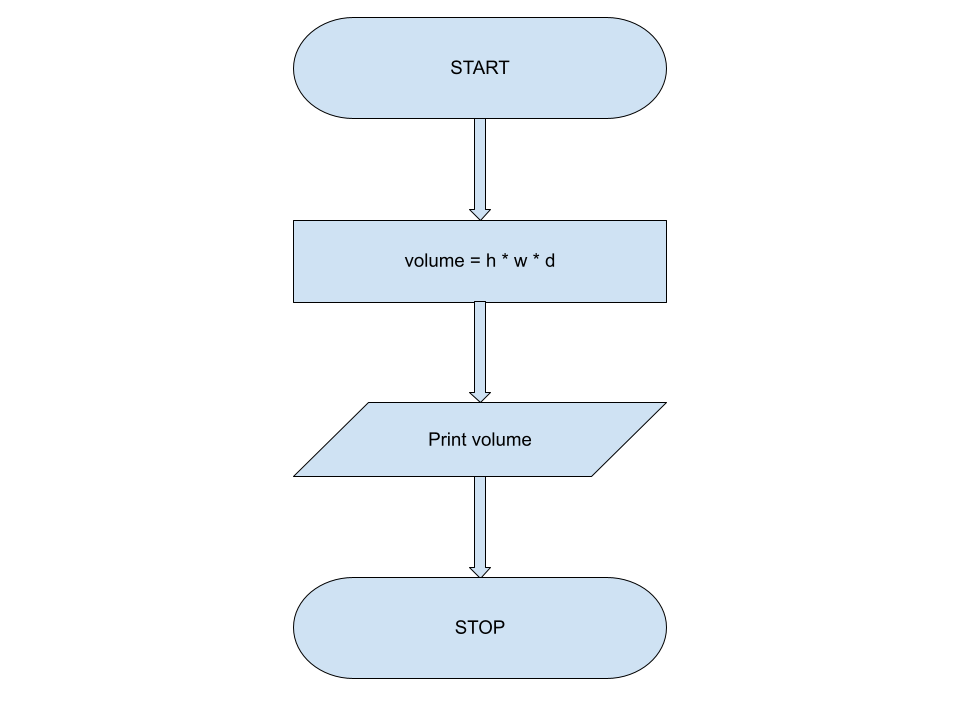
\includegraphics[width=1.0\textwidth]{Flowchart01.png}
\end{figure}
\newpage
\subsection{Code}
\inputminted{c}{q1.c}
\subsection{Output}
\begin{figure}[h]
    \centering
    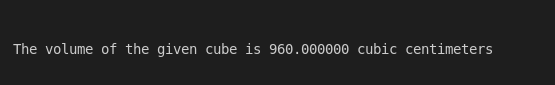
\includegraphics[width=1.0\textwidth]{1.png}
\end{figure}
\newpage
\section{}
\subsection{Algorithm}
\begin{enumerate}
    \item Input two numbers a and b
    \item Calculate the sum = a+b
    \item Subtract b from sum
    \item Divide sum by a
    \item Multiply last both results
    \item Display the answer
\end{enumerate}
\subsection{Flowchart}
\begin{figure}[h]
    \centering
    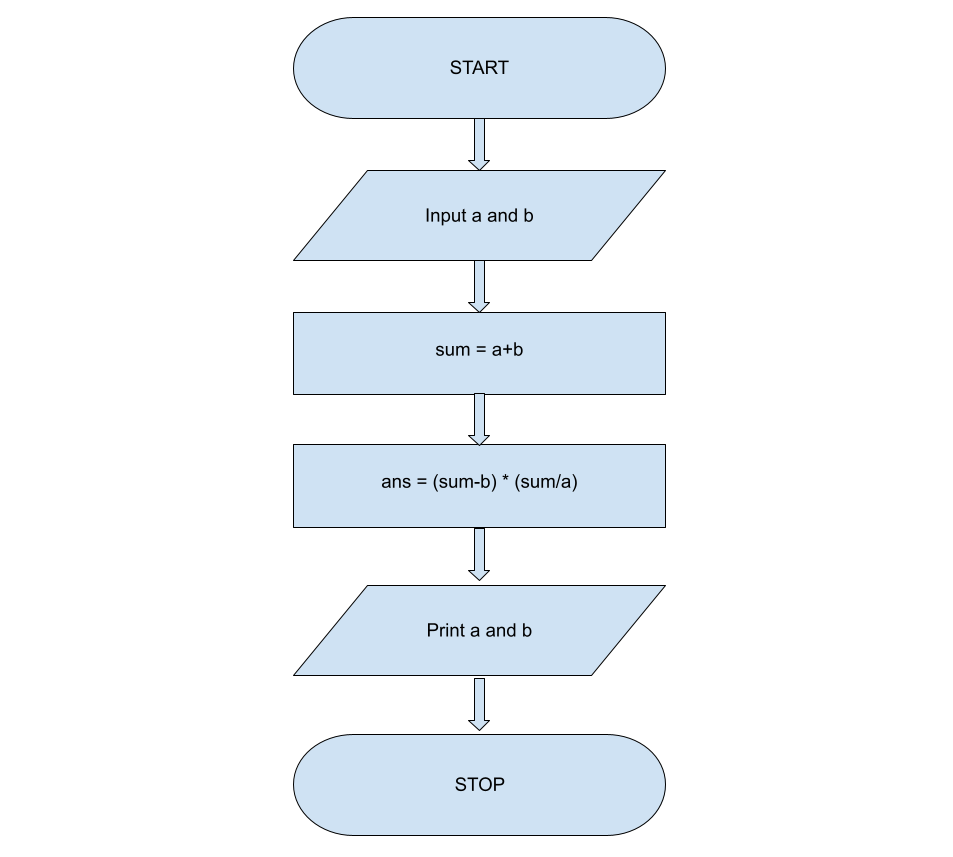
\includegraphics[width=1.0\textwidth]{Flowchart02.png}
\end{figure}
\newpage
\subsection{Code}
\inputminted{c}{q2.c}
\subsection{Output}
\begin{figure}[h]
    \centering
    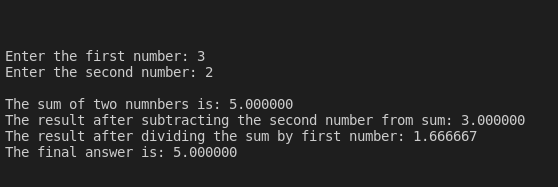
\includegraphics[width=1.0\textwidth]{2.png}
\end{figure}
\newpage
\section{}
\subsection{Algorithm}
\begin{enumerate}
    \item Use $sizeof()$ function to display the size of different data types
\end{enumerate}
\subsection{Flowchart}
\begin{figure}[h]
    \centering
    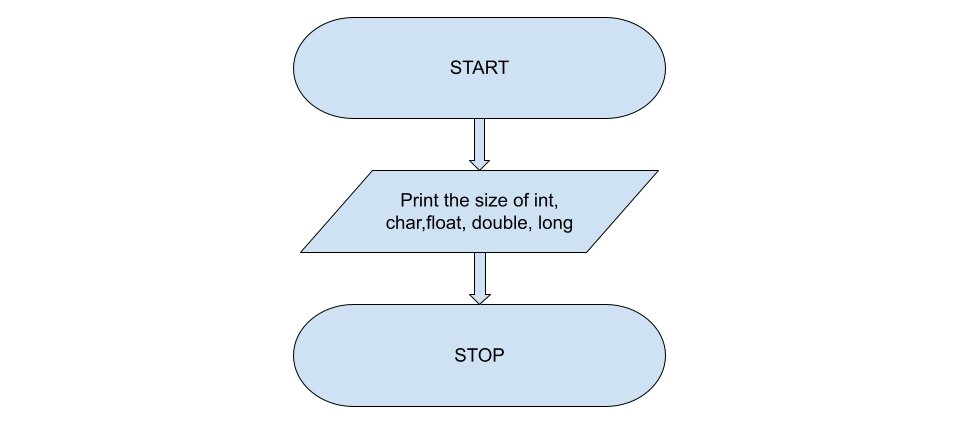
\includegraphics[width=1.0\textwidth]{Flowchart03.png}
\end{figure}
\newpage
\subsection{Code}
\inputminted{c}{q3.c}
\subsection{Output}
\begin{figure}[h]
    \centering
    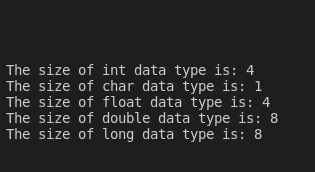
\includegraphics[width=1.0\textwidth]{3.png}
\end{figure}
\newpage
\section{}
\textbf{a}
\subsection{Algorithm}
\begin{enumerate}
    \item input 2 numbers
    \item Perform the basic arithmetic calculations: addition, subtraction, multiplication, division
    \item print the results
\end{enumerate}
\subsection{Flowchart}
\begin{figure}[h]
    \centering
    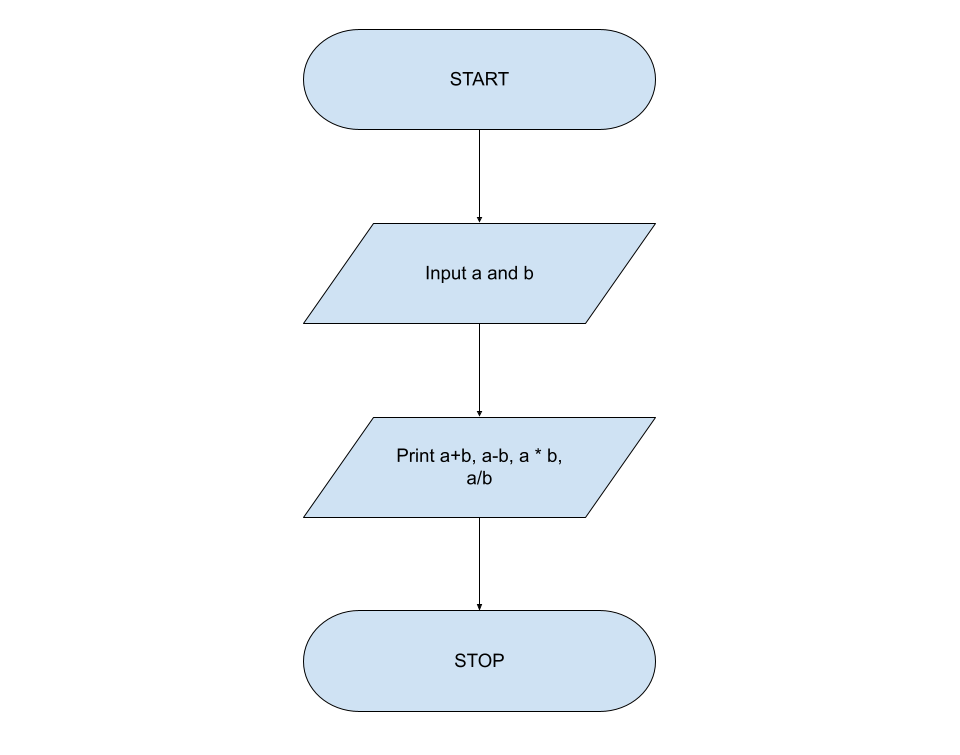
\includegraphics[width=1.0\textwidth]{Flowchart04a.png}
\end{figure}
\newpage
\subsection{Code}
\inputminted{c}{q4a.c}
\subsection{Output}
\begin{figure}[h]
    \centering
    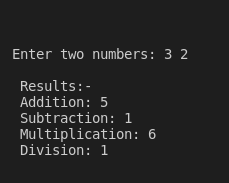
\includegraphics[width=1.0\textwidth]{4a.png}
\end{figure}\\ \newline
\newpage
\textbf{b}
\subsection{Algorithm}
\begin{enumerate}
    \item input two numbers
    \item add 10 to a
    \item divide the result by b
    \item print the final result
\end{enumerate}
\subsection{Flowchart}
\begin{figure}[h]
    \centering
    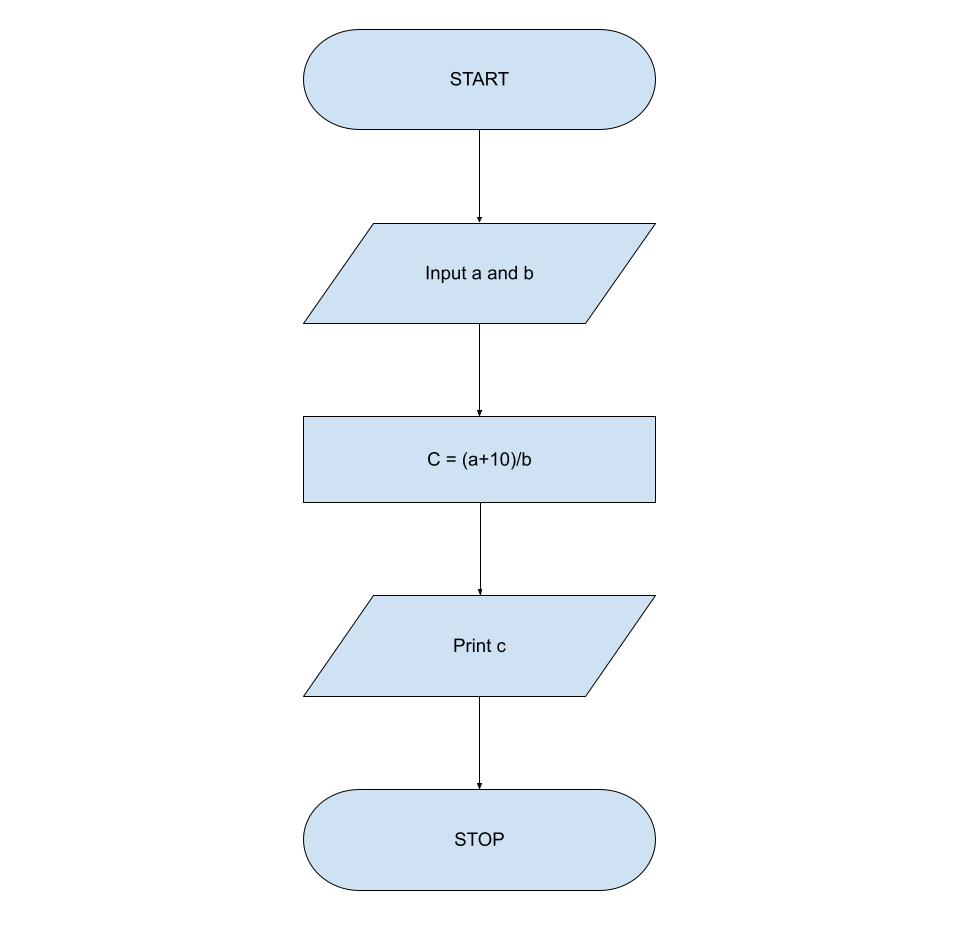
\includegraphics[width=1.0\textwidth]{Flowchart04b.png}
\end{figure}
\newpage
\subsection{Code}
\inputminted{c}{q4b.c}
\subsection{Output}
\begin{figure}[h]
    \centering
    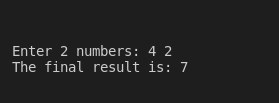
\includegraphics[width=1.0\textwidth]{4b.png}
\end{figure}\\ \newline
\newpage
\textbf{c}
\subsection{Algorithm}
\begin{enumerate}
    \item input two numbers
    \item check if a>b
    \item if true, print 1
    \item else print 0
\end{enumerate}
\subsection{Flowchart}
\begin{figure}[h]
    \centering
    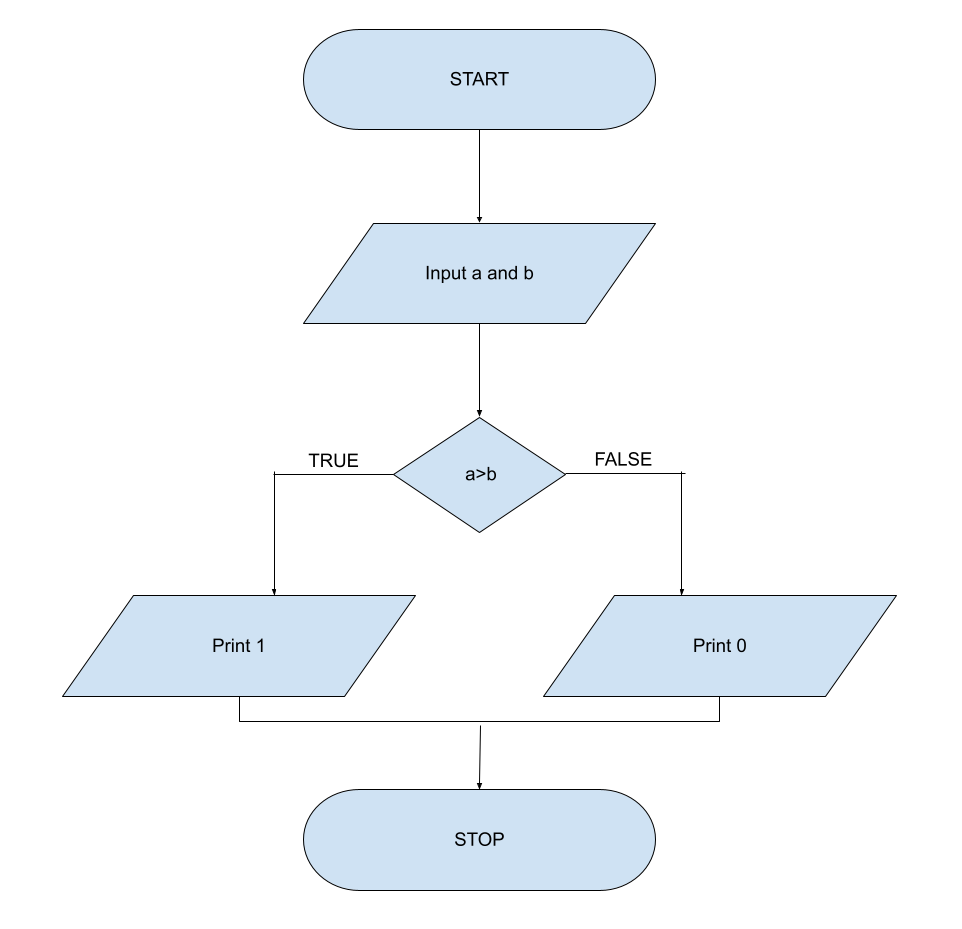
\includegraphics[width=1.0\textwidth]{Flowchart04c.png}
\end{figure}
\newpage
\subsection{Code}
\inputminted{c}{q4c.c}
\subsection{Output}
\begin{figure}[h]
    \centering
    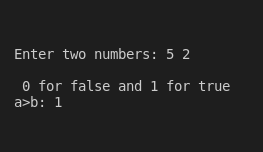
\includegraphics[width=1.0\textwidth]{4c.png}
\end{figure}\\ \newline
\newpage
\textbf{d}
\subsection{Algorithm}
\begin{enumerate}
    \item input three numbers
    \item check if a or b lie between 0 and 10
    \item check if x is not equal to 0
    \item if both conditions are true, print 1
    \item else, print 0
\end{enumerate}
\subsection{Flowchart}
\begin{figure}[h]
    \centering
    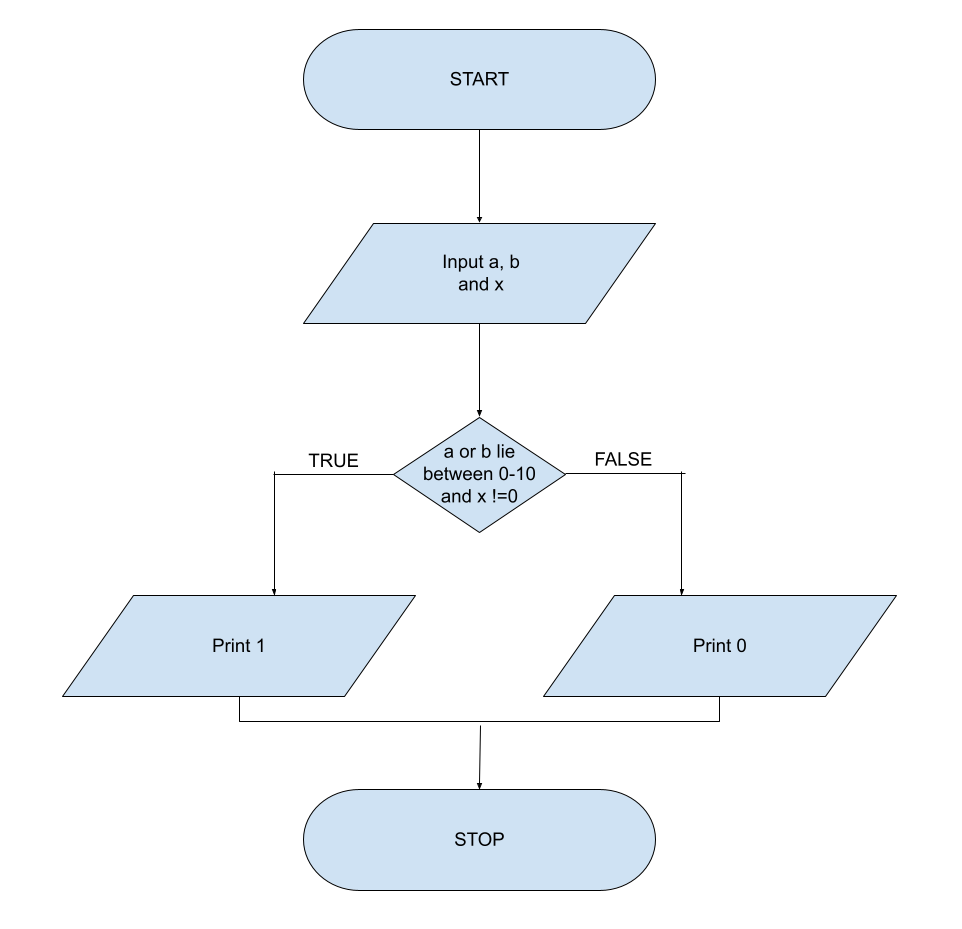
\includegraphics[width=1.0\textwidth]{Flowchart04d.png}
\end{figure}
\newpage
\subsection{Code}
\inputminted{c}{q4d.c}
\subsection{Output}
\begin{figure}[h]
    \centering
    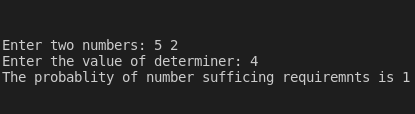
\includegraphics[width=1.0\textwidth]{4d.png}
\end{figure}\\ \newline
\newpage
\textbf{e}
\subsection{Algorithm}
\begin{enumerate}
    \item input two numbers
    \item check if a>b
    \item check if a is not equal to 0
    \item if both conditions are true, print 1
    \item else, print 0
\end{enumerate}
\subsection{Flowchart}
\begin{figure}[h]
    \centering
    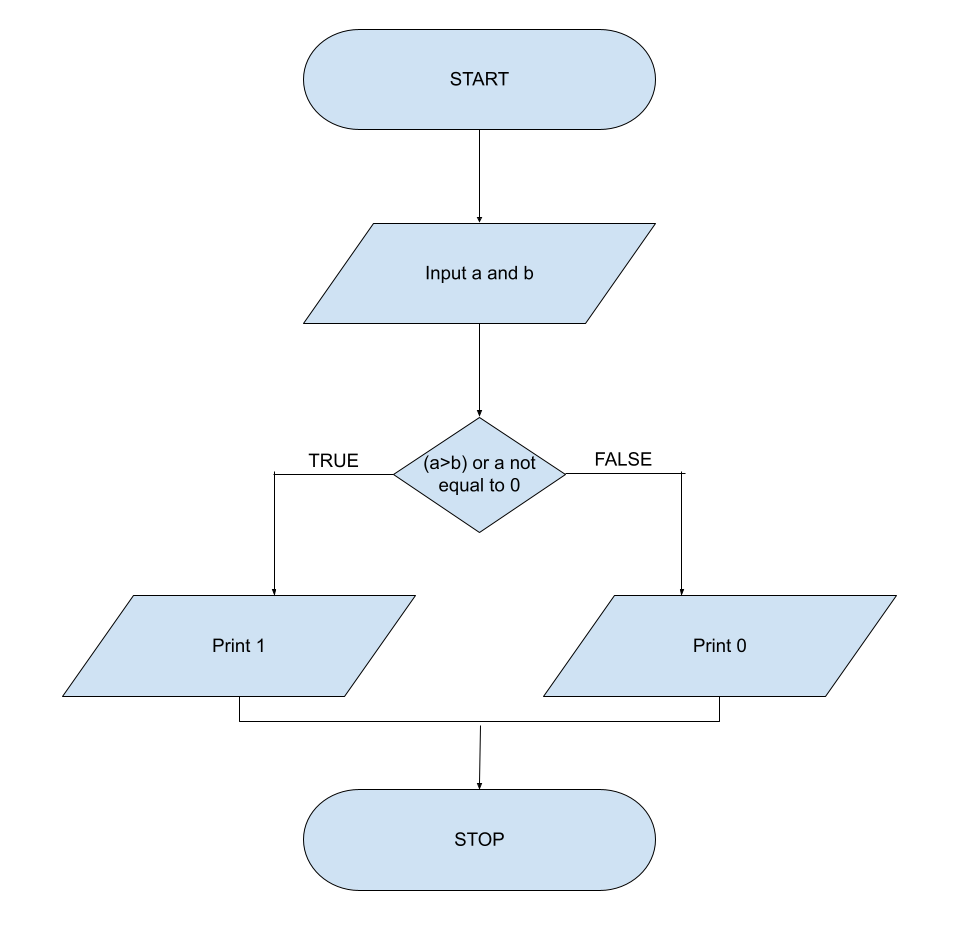
\includegraphics[width=1.0\textwidth]{Flowchart04e.png}
\end{figure}
\newpage
\subsection{Code}
\inputminted{c}{q4e.c}
\subsection{Output}
\begin{figure}[h]
    \centering
    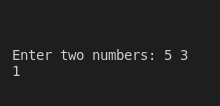
\includegraphics[width=1.0\textwidth]{4e.png}
\end{figure}
\newpage
\section{}
\subsection{Algorithm}
\begin{enumerate}
    \item input three sides of triangle
    \item calculate semi perimeter $s=(a+b+c)/2$
    \item calculate the area by Herone's formula: $A = \sqrt{s*(s-a)*(s-b)*(s-c)}$
    \item print area of triangle
\end{enumerate}
\subsection{Flowchart}
\begin{figure}[h]
    \centering
    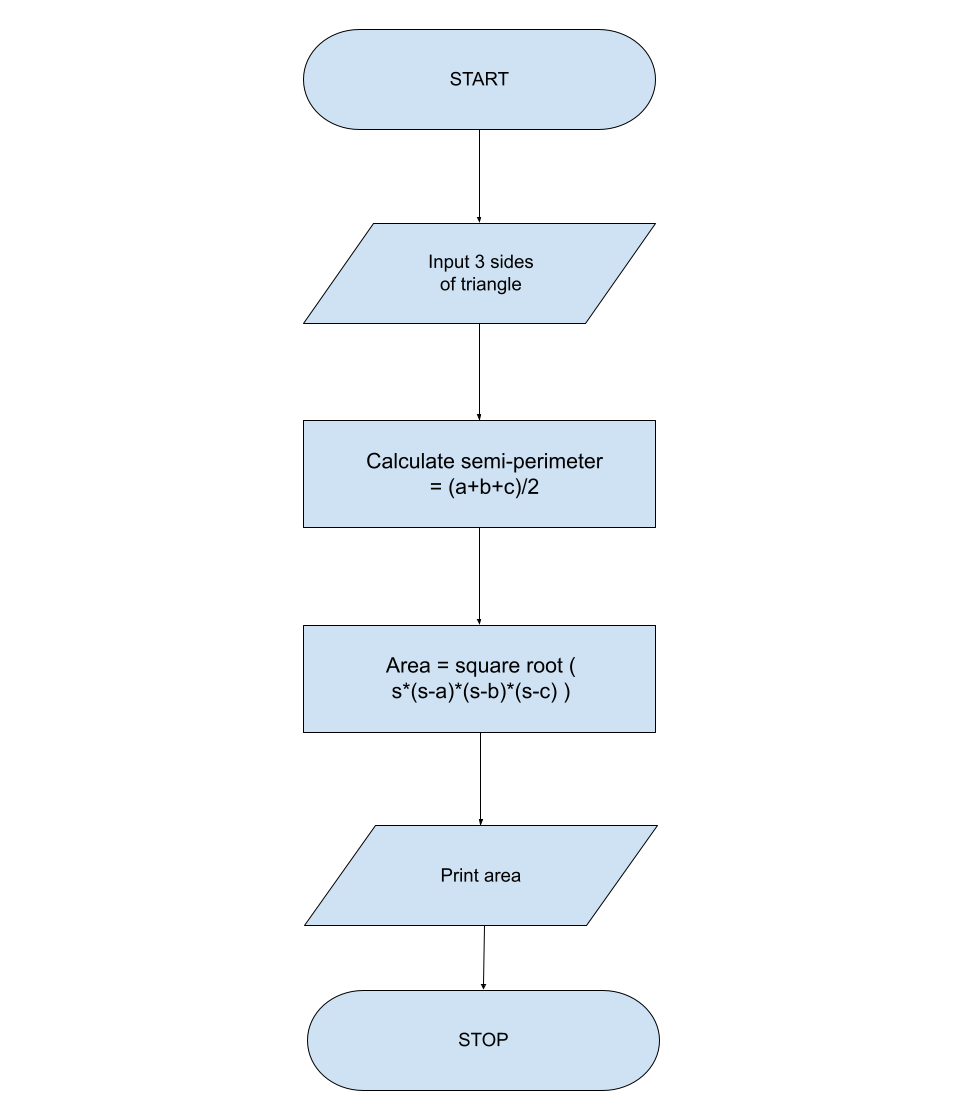
\includegraphics[width=1.0\textwidth]{Flowchart05.png}
\end{figure}
\newpage
\subsection{Code}
\inputminted{c}{q5.c}
\subsection{Output}
\begin{figure}[h]
    \centering
    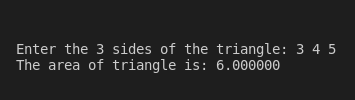
\includegraphics[width=1.0\textwidth]{5.png}
\end{figure}
\newpage
\section{}
\subsection{Algorithm}
\begin{enumerate}
    \item input the principal amount, rate, time
    \item calculate simple interest $SI=(P*R*T)/100$
    \item calculate compound interest $CI=(P(1+\frac{R}{100})^T)-P$
    \item Print simple and compound interest
\end{enumerate}
\subsection{Flowchart}
\begin{figure}[h]
    \centering
    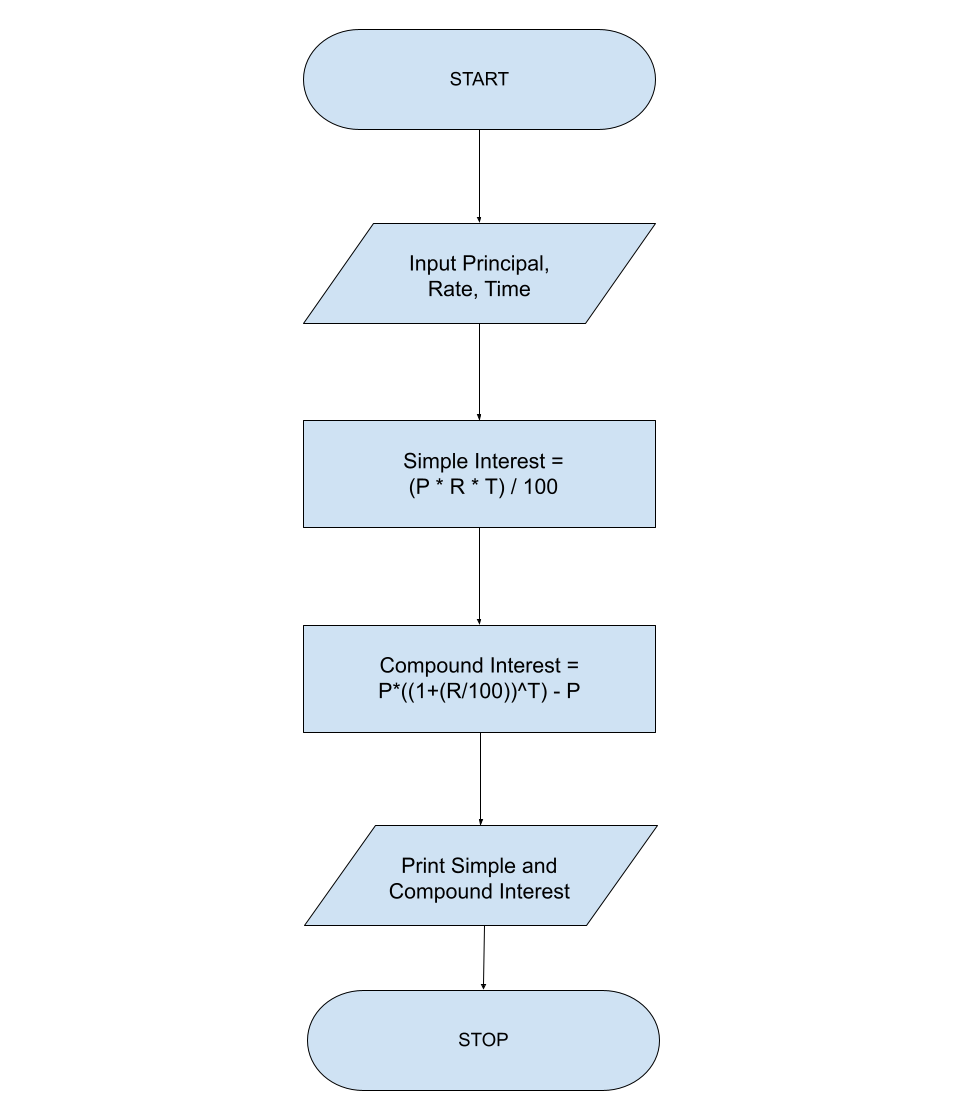
\includegraphics[width=1.0\textwidth]{Flowchart06.png}
\end{figure}
\newpage
\subsection{Code}
\inputminted{c}{q6.c}
\subsection{Output}
\begin{figure}[h]
    \centering
    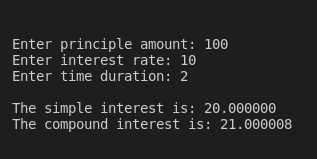
\includegraphics[width=1.0\textwidth]{6.png}
\end{figure}
\newpage
\section{}
\subsection{Algorithm}
\begin{enumerate}
    \item input the address
    \item print address
\end{enumerate}
\subsection{Flowchart}
\begin{figure}[h]
    \centering
    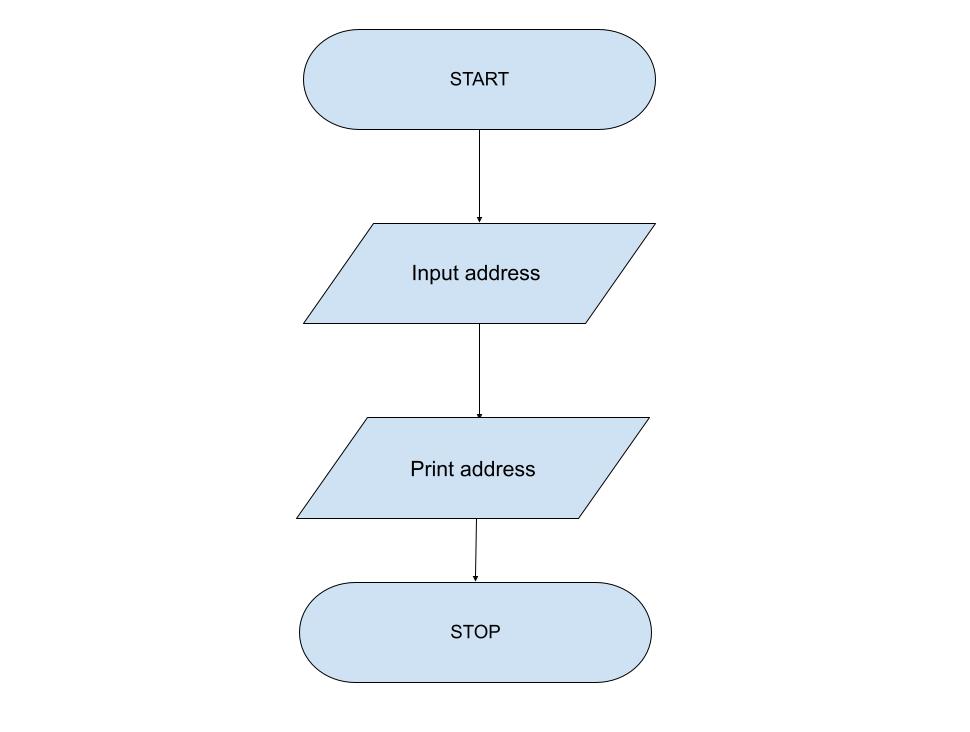
\includegraphics[width=1.0\textwidth]{Flowchart07.png}
\end{figure}
\newpage
\subsection{Code}
\inputminted{c}{q7.c}
\subsection{Output}
\begin{figure}[h]
    \centering
    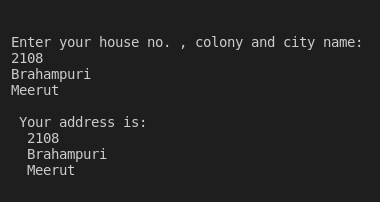
\includegraphics[width=1.0\textwidth]{7.png}
\end{figure}
\newpage
\section{}
\subsection{Algorithm}
\begin{enumerate}
    \item input basic pay
    \item calculate HRA by getting 10\% of the basic pay
    \item calculate TA by getting 5\% of the basic pay
    \item calculate total salary by adding basic pay, HRA and TA
    \item print total salary
\end{enumerate}
\subsection{Flowchart}
\begin{figure}[h]
    \centering
    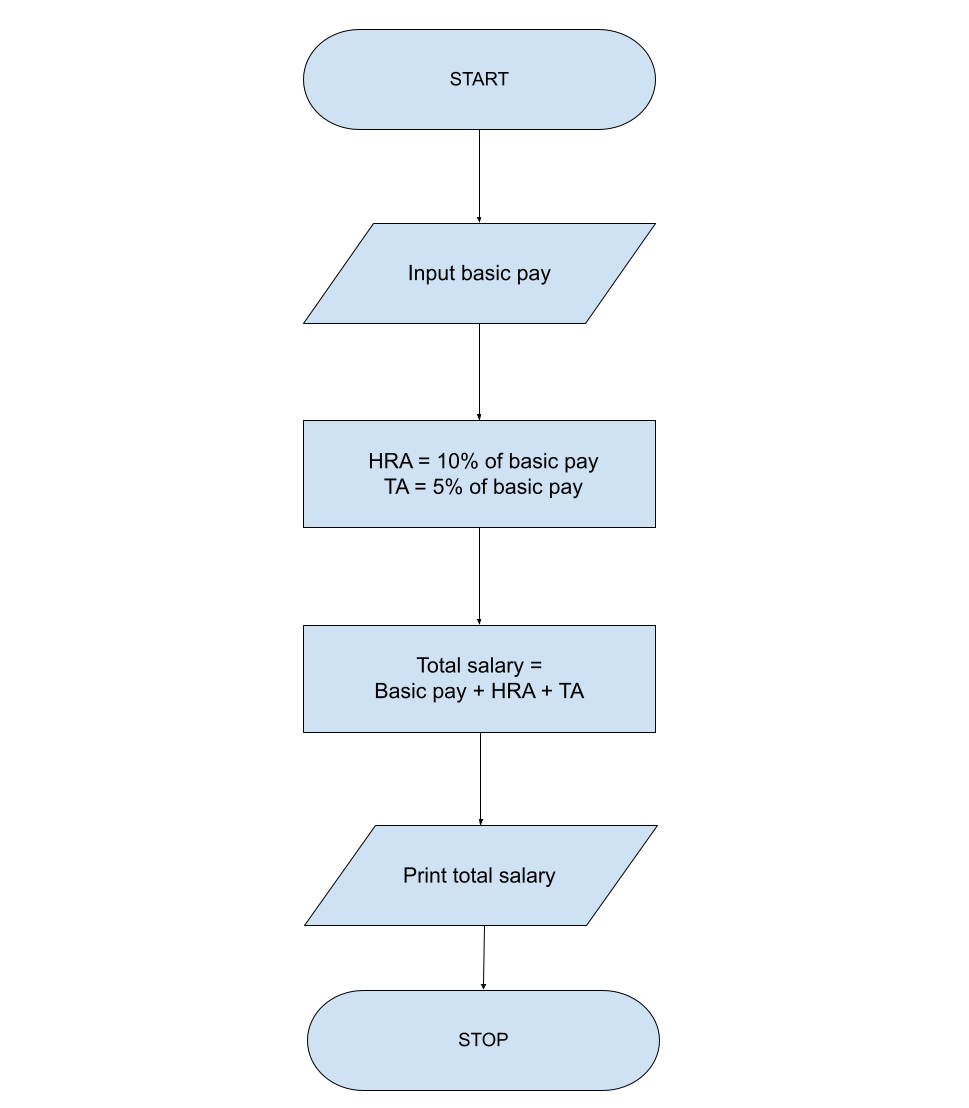
\includegraphics[width=1.0\textwidth]{Flowchart08.png}
\end{figure}
\newpage
\subsection{Code}
\inputminted{c}{q8.c}
\subsection{Output}
\begin{figure}[h]
    \centering
    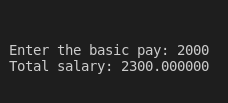
\includegraphics[width=1.0\textwidth]{8.png}
\end{figure}
\newpage
\section{}
\subsection{Algorithm}
\begin{enumerate}
    \item print a in two decimal places by using specifier \%.2e
    \item print a in four decimal places by using specifier \%.4e
    \item print a in eight decimal places by using specifier \%.8e
\end{enumerate}
\subsection{Flowchart}
\begin{figure}[h]
    \centering
    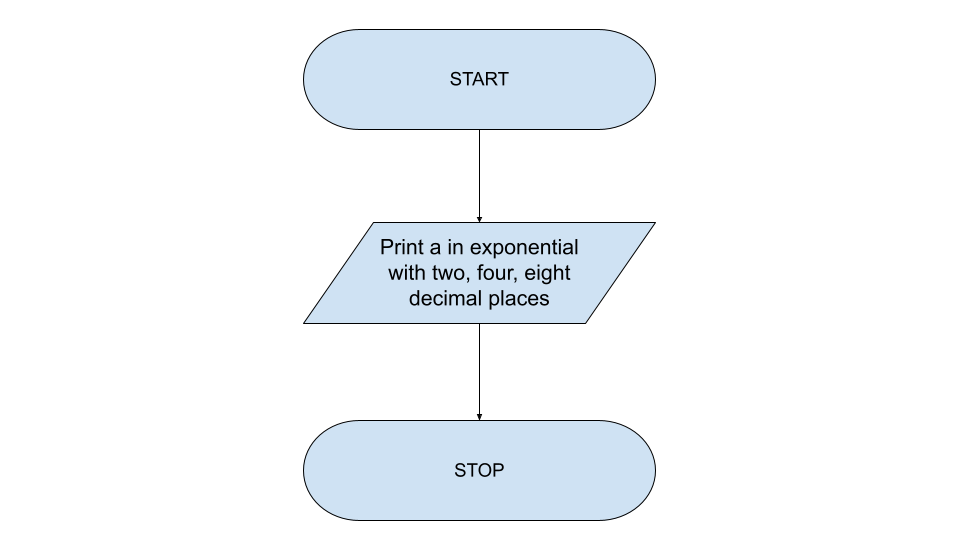
\includegraphics[width=1.0\textwidth]{Flowchart09.png}
\end{figure}
\newpage
\subsection{Code}
\inputminted{c}{q9.c}
\subsection{Output}
\begin{figure}[h]
    \centering
    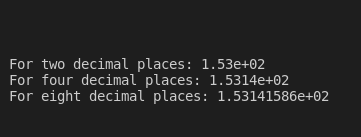
\includegraphics[width=1.0\textwidth]{9.png}
\end{figure}
\newpage
\section{}
\subsection{Algorithm}
\begin{enumerate}
    \item input two numbers a and b
    \item initialize a new variable c
    \item overwrite contents of c by those of a $c = a$
    \item overwrite contents of a by those of b $a = b$
    \item overwrite contents of b by those of c $b = c$
\end{enumerate}
\subsection{Flowchart}
\begin{figure}[h]
    \centering
    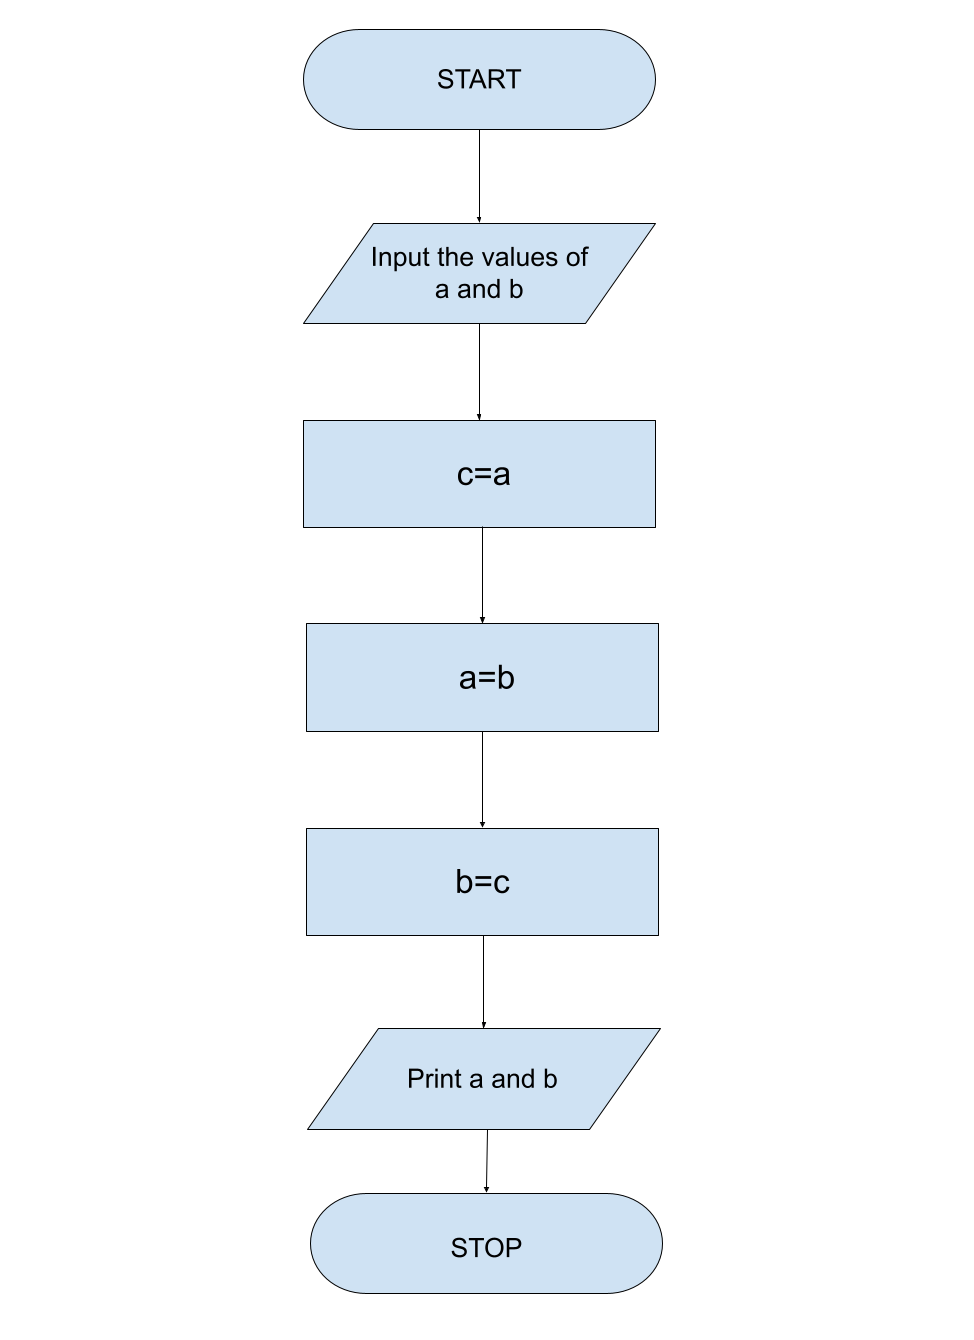
\includegraphics[width=0.8\textwidth]{Flowchart10.png}
\end{figure}
\newpage
\subsection{Code}
\inputminted{c}{q10.c}
\subsection{Output}
\begin{figure}[h]
    \centering
    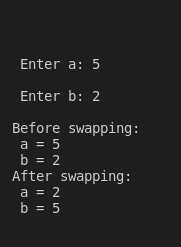
\includegraphics{10.png}
\end{figure}
\end{document}